\documentclass[11pt,a4paper]{article}

% ----- Packages -----
\usepackage[utf8]{inputenc}
\usepackage[T1]{fontenc}
\usepackage[spanish,es-tabla]{babel}
\usepackage{lmodern}
\usepackage[a4paper,margin=2.4cm]{geometry}
\usepackage{graphicx}
\usepackage{xcolor}
\usepackage{booktabs}
\usepackage{array}
\usepackage{caption}
\usepackage{subcaption}
\usepackage{listings}
\usepackage{tikz}
\usetikzlibrary{positioning, arrows.meta, fit, shapes.geometric, calc, shadows.blur, backgrounds}
\usepackage[most]{tcolorbox}
\usepackage{fancyhdr}
\setlength{\headheight}{22pt}
\usepackage{titlesec}
\usepackage[hidelinks,colorlinks=true,linkcolor=accent,urlcolor=accent,citecolor=accent]{hyperref}
\usepackage{enumitem}
\usepackage{microtype}

% ----- Colors (paleta accent + grises) -----
\definecolor{accent}{HTML}{1F6FEB}
\definecolor{accent2}{HTML}{0A8754}
\definecolor{warn}{HTML}{D1351A}
\definecolor{bg}{HTML}{F6F8FA}
\definecolor{bgbox}{HTML}{EDF2F7}
\definecolor{rule}{HTML}{D0D7DE}
\definecolor{ink}{HTML}{1F2328}
\definecolor{muted}{HTML}{57606A}
\definecolor{good}{HTML}{1A7F37}
\definecolor{jsonkey}{HTML}{0550AE}
\definecolor{jsonval}{HTML}{0A3069}
\definecolor{jsonstr}{HTML}{0A8754}

\color{ink}

% ----- Header/footer -----
\pagestyle{fancy}
\fancyhf{}
\fancyhead[L]{\small\color{muted}\textsc{TP3 — Perceptrones}}
\fancyhead[R]{\small\color{muted}ITBA · 1Q 2026}
\fancyfoot[C]{\small\color{muted}\thepage}
\renewcommand{\headrulewidth}{0.4pt}
\renewcommand{\headrule}{\hbox to\headwidth{\color{rule}\leaders\hrule height \headrulewidth\hfill}}

% ----- Section style -----
\titleformat{\section}
  {\Large\bfseries\color{accent}}
  {\thesection.}{0.6em}{}
\titleformat{\subsection}
  {\large\bfseries\color{ink}}
  {\thesubsection}{0.6em}{}

% ----- TCB boxes -----
\newtcolorbox{insight}[1][]{
  enhanced, breakable,
  colback=bgbox, colframe=accent,
  boxrule=0pt, leftrule=4pt,
  arc=2pt, outer arc=0pt,
  left=10pt, right=10pt, top=8pt, bottom=8pt,
  fonttitle=\bfseries\color{accent},
  title={\faIcon{lightbulb} Insight},
  #1
}
\newtcolorbox{caveat}[1][]{
  enhanced, breakable,
  colback=bgbox, colframe=warn,
  boxrule=0pt, leftrule=4pt,
  arc=2pt, outer arc=0pt,
  left=10pt, right=10pt, top=8pt, bottom=8pt,
  fonttitle=\bfseries\color{warn},
  #1
}
\newtcolorbox{takeaway}[1][]{
  enhanced, breakable,
  colback=accent2!8, colframe=accent2,
  boxrule=0pt, leftrule=4pt,
  arc=2pt, outer arc=0pt,
  left=10pt, right=10pt, top=8pt, bottom=8pt,
  fonttitle=\bfseries\color{accent2},
  #1
}

% ----- listings -----
\lstdefinelanguage{json}{
    basicstyle=\ttfamily\small\color{ink},
    string=[s]{"}{"},
    stringstyle=\color{jsonstr},
    morestring=[b]",
    morecomment=[l]{//},
    commentstyle=\color{muted}\itshape,
    keywords={true,false,null},
    keywordstyle=\color{warn}\bfseries,
    showstringspaces=false,
    breaklines=true,
    backgroundcolor=\color{bg},
    frame=none,
    framexleftmargin=10pt,
    xleftmargin=10pt,
}
\lstset{
    basicstyle=\ttfamily\small,
    backgroundcolor=\color{bg},
    breaklines=true,
    showstringspaces=false,
    captionpos=b,
}

% ----- Custom commands -----
\newcommand{\ok}{\textcolor{good}{\ding{52}}}
\newcommand{\nok}{\textcolor{warn}{\ding{56}}}
\newcommand{\code}[1]{\texttt{\textcolor{accent}{#1}}}
\newcommand{\file}[1]{\texttt{\small #1}}
\usepackage{pifont}

% Shadow utility
\tikzset{
  every shadow/.style={shadow xshift=0.6pt, shadow yshift=-0.6pt, opacity=0.18},
}

% ===================================================================
\begin{document}

% =============== COVER ===============
\begin{titlepage}
\thispagestyle{empty}
\begin{tikzpicture}[remember picture, overlay]
  % Background gradient bar on the left
  \fill[accent!90] (current page.north west) rectangle ($(current page.south west) + (1.6,0)$);
  \fill[accent!60] ($(current page.north west) + (1.6,0)$) rectangle ($(current page.south west) + (1.85,0)$);
  % Decorative dots
  \foreach \x in {0,...,16} {
    \foreach \y in {0,...,24} {
      \fill[white!85!accent, opacity=0.4]
        ($(current page.north west) + (0.18 + 0.085*\x, -0.18 - 0.085*\y)$) circle (0.35pt);
    }
  }
\end{tikzpicture}

\vspace*{3cm}
\begin{flushleft}
{\fontsize{42}{48}\selectfont\bfseries\color{ink}TP3}\\[0.4em]
{\fontsize{32}{38}\selectfont\bfseries\color{accent}Perceptrones}\\[0.6em]
{\Large\color{muted}Implementación desde cero, con NumPy.}\\[2em]

\rule{\linewidth}{0.4pt}\\[0.6em]
{\large\textbf{Sistemas de Inteligencia Artificial} \textcolor{muted}{·}\ Trabajo Práctico 3}\\[0.3em]
{\large\color{muted}ITBA · Primer Cuatrimestre 2026}\\[3em]

\begin{tabular}{@{}ll@{}}
  \large\bfseries Engine MLP genérico & \code{mlp/} \\
  \large\bfseries Ejercicio 0 — Validación & \code{ejercicio0/} \\
  \large\bfseries Ejercicio 1 — Fraud detection & \code{ejercicio1/} \quad\textit{(Tomás)} \\
  \large\bfseries Ejercicio 2 — Clasificación de dígitos & \code{ejercicio2/} \\
  \large\bfseries Ejercicio 3 — Dígitos $\geq 98\%$ & \code{ejercicio3/} \\
\end{tabular}
\end{flushleft}

\vfill
\begin{flushleft}
\rule{\linewidth}{0.4pt}\\[0.4em]
\textcolor{muted}{\small Documento companion de \code{docs/guia\_compañeros.md}.\\
Repositorio: \texttt{github.com/pi-na/SIA-TP3} · branch \texttt{tp3-mlp}.}
\end{flushleft}
\end{titlepage}

% =============== ABSTRACT ===============
\section*{Resumen ejecutivo}
\addcontentsline{toc}{section}{Resumen ejecutivo}

Este TP construye un \textbf{módulo MLP genérico} (\code{mlp/}, NumPy puro) y resuelve sobre él los Ejercicios 0, 2 y 3. La filosofía es separar el \textbf{engine} de los \textbf{experimentos}: cada experimento es un \code{config.json} \(\rightarrow\) una corrida \(\rightarrow\) una carpeta de outputs (CSVs + npz) \(\rightarrow\) plots para slides.

\medskip
La metodología en Ej2 fue \textbf{coarse-to-fine en dos fases}:
\begin{itemize}[leftmargin=1.4em, itemsep=2pt]
  \item \textbf{Fase 1} (k\_folds$=$1, exploratoria): sweeps secuenciales arch \(\to\) opt \(\to\) LR \(\to\) batch. Cada sub-fase usa el ganador del anterior. Reduce el espacio de búsqueda de $\mathcal{O}(n^4)$ a $\mathcal{O}(4n)$.
  \item \textbf{Fase 2} (k\_folds$=$5, validación): one-at-a-time sobre el \code{base.json} consolidado. Comparativas limpias para presentación.
  \item \textbf{Final eval}: una única evaluación contra \code{digits\_test.csv}.
\end{itemize}

El descubrimiento clave fue un \textbf{distribution shift} entre \code{digits.csv} y \code{digits\_test.csv}: el modelo Ej2 con val K$=$5 de \textbf{96.22\%} caía a \textbf{86.30\%} en test. Eso motivó el Ej3, donde simplemente concatenar \code{more\_digits.csv} levantó el test a \textbf{96.36\%} (\(+10\)pp). Pack C (L2 + augmentation gaussiana) llevó al ganador a \textbf{96.88\%}.

\begin{caveat}
\textbf{Target del Ej3 (\(\geq 98\%\)) no alcanzado.} Mejor obtenido: \textbf{96.88\%} (faltan 1.12\,pp). El análisis identifica como hipótesis principal que el shift residual en \code{digits\_test.csv} no se captura con \emph{noise} isotrópico — habría que augmentar con transformaciones geométricas (rotación, traslación). Detalle en §\ref{sec:ej3}.
\end{caveat}

\tableofcontents
\bigskip\hrule\bigskip

% =============== INTRO ===============
\section{Introducción y filosofía}

\subsection{Restricciones del enunciado}
La consigna pide implementar perceptrones \textbf{desde cero}: nada de \texttt{sklearn} estimators, ni \texttt{PyTorch}/\texttt{TensorFlow} como capas. Solo NumPy para operaciones matriciales, Pandas para cargar datos, Matplotlib para plots. Esto fuerza a tener una buena ingeniería del backprop, los optimizadores y la pipeline de datos.

\subsection{Decisión arquitectural: un único engine}
En vez de armar tres scripts independientes (uno por ejercicio), construimos un \textbf{módulo \code{mlp/}} reutilizable y usamos \textbf{configs JSON} para cada experimento. Beneficios:
\begin{itemize}[leftmargin=1.4em, itemsep=2pt]
  \item Una sola codebase, un solo set de tests (78 tests verde).
  \item Comparar entre ejercicios es trivial (mismo binario, otro JSON).
  \item Pack C (regularización del Ej3) se agrega via \code{regularization} en el config sin tocar la pipeline.
\end{itemize}

\begin{insight}
La validación (XOR, AND) usa \emph{exactamente el mismo código} que la clasificación de dígitos. Si rompe la red para 4 puntos, también está rota para 12.000.
\end{insight}

% =============== ENGINE ===============
\section{El engine \code{mlp/}}

\subsection{Anatomía}

\begin{center}
\begin{tikzpicture}[
    every node/.style={font=\small},
    block/.style={
      draw=accent, fill=bg,
      rounded corners=3pt, minimum width=3.6cm, minimum height=1.0cm,
      drop shadow={shadow xshift=0.6pt, shadow yshift=-0.6pt, opacity=0.18}
    },
    title/.style={font=\small\bfseries\color{accent}},
    arrow/.style={-{Latex[length=2mm]}, accent, thick}
]

  \node[block] (forward) {\code{forward(X, training)}};
  \node[block, below=0.6cm of forward] (backward) {\code{backward(X, y, cache)}};
  \node[block, below=0.6cm of backward] (fit) {\code{fit(X\_tr, y\_tr, X\_val, y\_val)}};
  \node[block, below=0.6cm of fit] (predict) {\code{predict / predict\_proba}};

  \node[block, right=2.4cm of forward, fill=accent2!10, draw=accent2] (act) {Activations};
  \node[block, below=0.4cm of act, fill=accent2!10, draw=accent2] (loss) {Losses};
  \node[block, below=0.4cm of loss, fill=accent2!10, draw=accent2] (init) {Initializers};
  \node[block, below=0.4cm of init, fill=accent2!10, draw=accent2] (opt) {Optimizers};

  \draw[arrow] (forward) -- (backward);
  \draw[arrow] (backward) -- (fit);
  \draw[arrow] (fit) -- (predict);

  \draw[arrow, dashed, opacity=0.6] (act) -- (forward);
  \draw[arrow, dashed, opacity=0.6] (loss) -- (backward);
  \draw[arrow, dashed, opacity=0.6] (init) -- (forward);
  \draw[arrow, dashed, opacity=0.6] (opt) -- (fit);

  \node[title, above=0.2cm of forward] (t1) {Pipeline};
  \node[title, above=0.2cm of act] (t2) {Componentes intercambiables};
\end{tikzpicture}
\end{center}

\subsection{Componentes}

\begin{center}
\begin{tabular}{@{}lll@{}}
\toprule
\textbf{Archivo} & \textbf{Responsabilidad} & \textbf{Variantes} \\
\midrule
\file{mlp/network.py}      & Clase \code{MLP}: forward, backward, fit, save, load & --- \\
\file{mlp/activations.py}  & Funciones y derivadas                  & sigmoid, tanh, relu, identity, softmax \\
\file{mlp/losses.py}       & Loss + gradiente                        & MSE, BCE, cross\_entropy \\
\file{mlp/initializers.py} & Inicializadores                         & uniform, He, Xavier, \emph{auto} \\
\file{mlp/optimizers.py}   & Optimizadores                           & SGD, Momentum, Adam \\
\file{mlp/data.py}         & Loaders y mini-batch iteration          & --- \\
\file{mlp/metrics.py}      & Métricas multiclase                     & accuracy, macro/weighted F1, confusion \\
\file{mlp/train.py}        & CLI config-driven con K-fold + workers  & --- \\
\bottomrule
\end{tabular}
\end{center}

\subsection{Bias trick y forward}
Cada peso \(W^{(l)}\) tiene shape \((n_{l+1},\, n_l + 1)\): la columna 0 es el bias. Antes de cada \texttt{matmul}, \code{\_add\_bias\_column} prepende una columna de 1's. Esto evita un parámetro \(b\) separado y simplifica el backprop.

El cache que devuelve \code{forward} es una lista de tuplas \((z_l,\, a_l^{\text{pre}},\, \text{mask}_l)\). El tercer elemento (\code{mask}) es para inverted dropout, igual a \code{None} en eval.

\subsection{Pack C — regularización configurable}

\begin{lstlisting}[language=json, caption={Bloque \texttt{regularization} de un config Pack C}, captionpos=b]
"regularization": {
  "l2": 1e-4,
  "dropout": 0.2,
  "lr_schedule": {"type": "step", "decay": 0.5, "every": 10},
  "augmentation": {"type": "gaussian_noise", "sigma": 0.05}
}
\end{lstlisting}

\begin{itemize}[leftmargin=1.4em, itemsep=2pt]
  \item \textbf{L2}: weight decay con \(\lambda = 10^{-4}\). No penaliza la columna de bias.
  \item \textbf{Dropout}: inverted dropout en hidden layers, training-only. \(\text{mask}\) se cachea para que el backward use \texttt{chain rule} correctamente.
  \item \textbf{LR schedule}: step decay multiplicativo cada \texttt{every} epochs.
  \item \textbf{Augmentation}: \emph{Gaussian noise} aditivo pre-batch sobre el input.
\end{itemize}

\begin{takeaway}
La elección de implementar Pack C \emph{vía config} (en lugar de scripts separados) significa que la misma pipeline corre Ej2 y Ej3 sin cambios — la única diferencia entre \file{ejercicio2/configs/base.json} y \file{ejercicio3/configs/pack\_c/l2\_aug.json} son los campos \texttt{extra\_csv\_paths} y \texttt{regularization}.
\end{takeaway}

% =============== EJ0 ===============
\section{Ejercicio 0 — Validación}

\subsection{Step perceptron y AND}
Implementación bipolar (\(\{-1,+1\}\)). 4 muestras, output esperado \([-1,-1,-1,+1]\). Tests verifican convergencia exacta (error \(=0\)) en el mismo orden que el enunciado.

\subsection{MLP en XOR}
Configs \file{xor\_2\_2\_1.json} (mínima) y \file{xor\_2\_3\_2\_1.json} (con capa extra). Ambas convergen a \(\text{train\_loss} < 0.1\) en pocas epochs. Estos tests son la red de seguridad del engine: si rompe el backprop, XOR deja de converger.

\begin{lstlisting}[language=json, caption={\file{xor\_2\_2\_1.json} — la arquitectura mínima que resuelve XOR}, captionpos=b]
{
  "architecture": {"layer_sizes": [2, 2, 1], "activations": ["tanh", "tanh"]},
  "training":     {"loss": "mse", "optimizer": {"name": "sgd", "lr": 0.1},
                   "epochs": 2000, "batch_size": 4}
}
\end{lstlisting}

% =============== EJ2 ===============
\section{Ejercicio 2 — Clasificación de dígitos}\label{sec:ej2}

\subsection{Datos}
\begin{itemize}[leftmargin=1.4em, itemsep=2pt]
  \item Train: \file{digits.csv} — 12.449 muestras, 10 clases.
  \item Test (producción): \file{digits\_test.csv} — 2.498 muestras. \textbf{No se toca durante búsqueda de HP.}
  \item Cada muestra es un vector de 784 floats en \([0,1]\) (28\(\times\)28 flatten).
\end{itemize}

\subsection{Workflow disciplinado}

\begin{center}
\begin{tikzpicture}[
  every node/.style={font=\small},
  phase/.style={
    draw=accent, fill=bg, rounded corners=3pt,
    minimum width=4.0cm, minimum height=1.5cm, align=center,
    drop shadow={shadow xshift=0.6pt, shadow yshift=-0.6pt, opacity=0.18}
  },
  result/.style={
    draw=accent2, fill=accent2!8, rounded corners=3pt,
    minimum width=4.0cm, minimum height=1.5cm, align=center,
    drop shadow={shadow xshift=0.6pt, shadow yshift=-0.6pt, opacity=0.18}
  },
  arrow/.style={-{Latex[length=3mm]}, accent, very thick}
]
  \node[phase] (f1) {\textbf{Fase 1}\\\small k\_folds$=$1\\\small arch \(\to\) opt \(\to\) LR \(\to\) batch};
  \node[result, right=1.6cm of f1] (base) {\textbf{base.json}\\\small ganador consolidado};
  \node[phase, right=1.6cm of base] (f2) {\textbf{Fase 2}\\\small k\_folds$=$5\\\small one-at-a-time};
  \node[result, below=1.0cm of base] (final) {\textbf{final\_eval}\\\small contra digits\_test.csv\\\small (UNA sola vez)};

  \draw[arrow] (f1) -- (base);
  \draw[arrow] (base) -- (f2);
  \draw[arrow] (f2.south) -- ++(0,-0.3) -| (final.east);
  \draw[arrow, dashed] (base.south) -- (final.north);
\end{tikzpicture}
\end{center}

\subsection{Fase 1 — sweeps secuenciales}

\begin{center}
\begin{tabular}{@{}llrrr@{}}
\toprule
\textbf{Sweep} & \textbf{Ganador} & \textbf{val\_acc} & \textbf{best\_ep} & \textbf{Comentario} \\
\midrule
1.1 Arquitectura  & \texttt{[784,100,50,10]}     & 0.9674 & 7  & Empate técnico con \texttt{[784,128,64,10]}, elegido por parsimonia \\
1.2 Optimizador   & \texttt{adam}, lr$=$0.001    & 0.9674 & 7  & sgd 94.81\% (no convergió en 50 ep) \\
1.3 Learning rate & \texttt{0.001}               & 0.9674 & 7  & lr$=$0.0001 no converge; \(\geq\)0.005 overshoot \\
1.4 Batch size    & \texttt{16}                  & 0.9674 & 3  & best macro\_f1 (0.8646), 12s — el más rápido por bastante \\
\bottomrule
\end{tabular}
\end{center}

El \textbf{\code{base.json}} consolidado corre con K-fold$=$5 antes de Fase 2, dando un baseline confiable: \(\text{val\_acc} = 0.9622 \pm 0.0043\).

\subsection{Fase 2 — one-at-a-time con K-fold$=$5}

\begin{figure}[h]
\centering
\begin{subfigure}{0.48\textwidth}
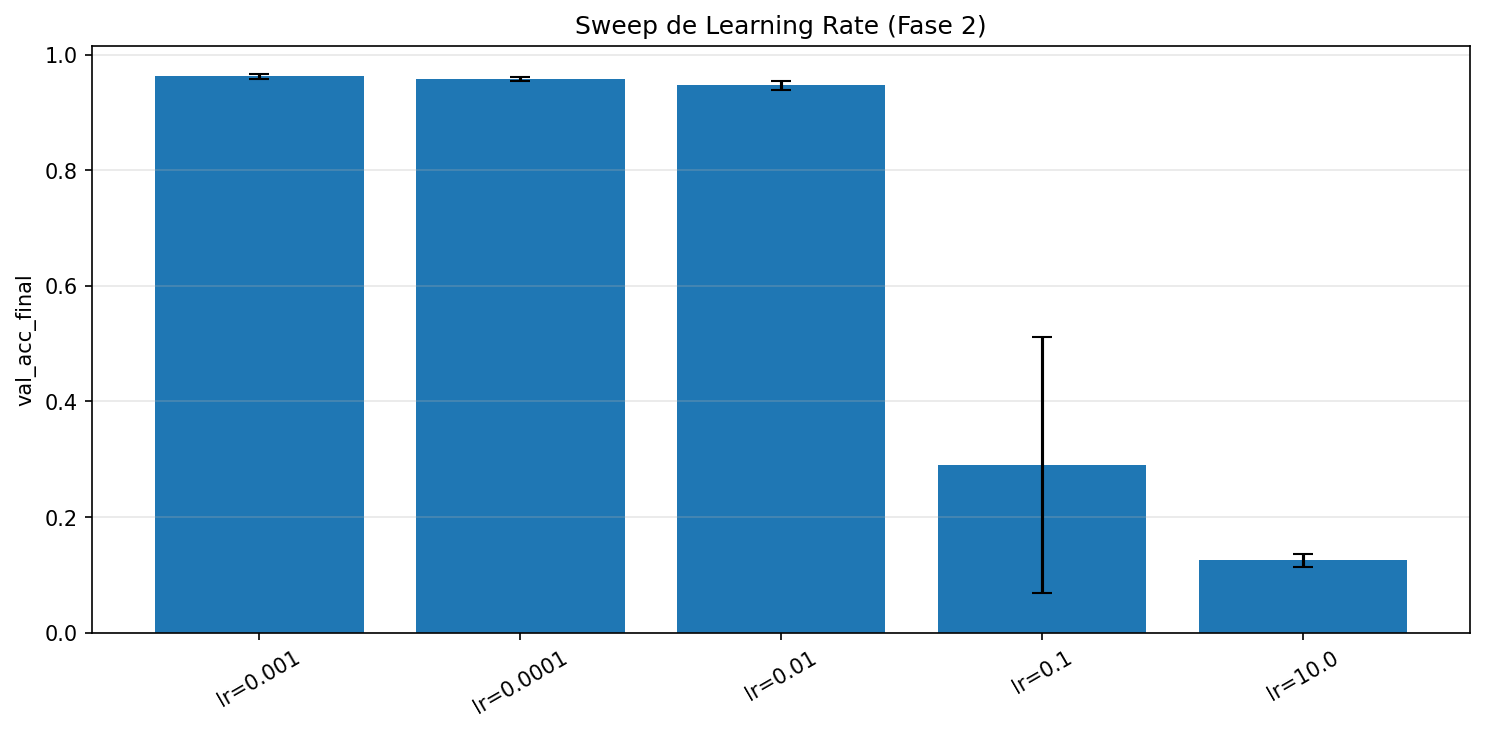
\includegraphics[width=\linewidth]{../ejercicio2/presentacion/02_sweep_lr.png}
\caption{Sweep de Learning Rate}
\end{subfigure}\hfill
\begin{subfigure}{0.48\textwidth}
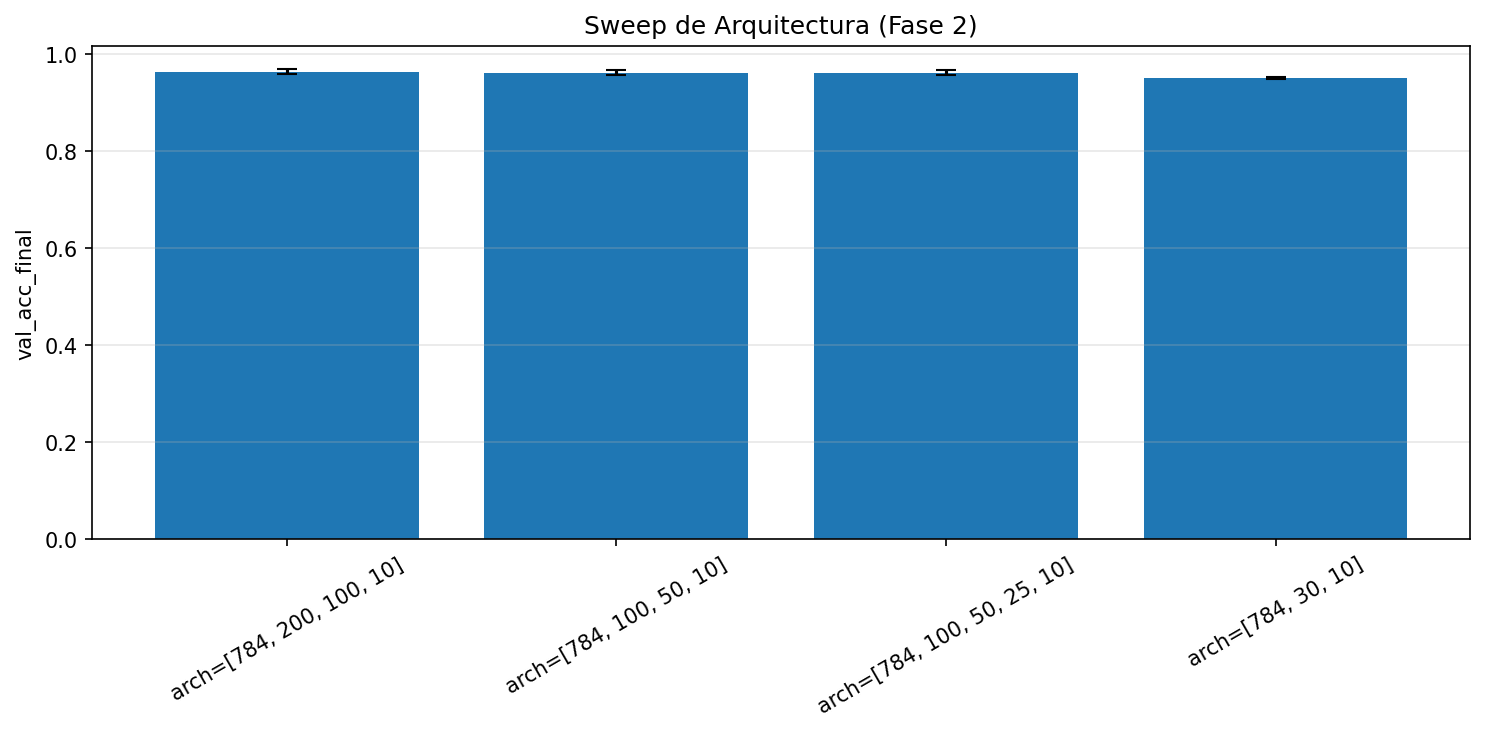
\includegraphics[width=\linewidth]{../ejercicio2/presentacion/03_sweep_arch.png}
\caption{Sweep de Arquitectura}
\end{subfigure}
\\[0.6em]
\begin{subfigure}{0.48\textwidth}
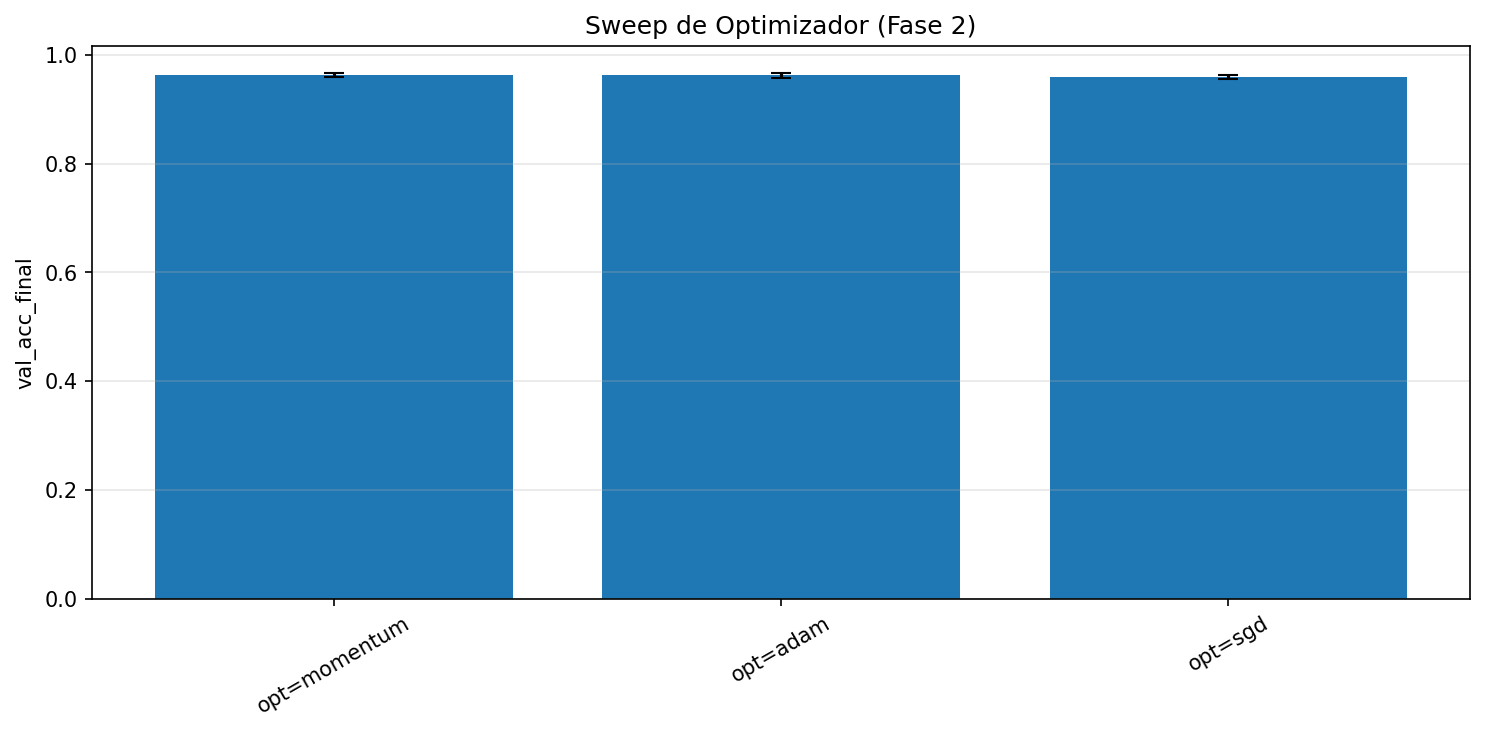
\includegraphics[width=\linewidth]{../ejercicio2/presentacion/06_sweep_opt.png}
\caption{Sweep de Optimizador}
\end{subfigure}\hfill
\begin{subfigure}{0.48\textwidth}
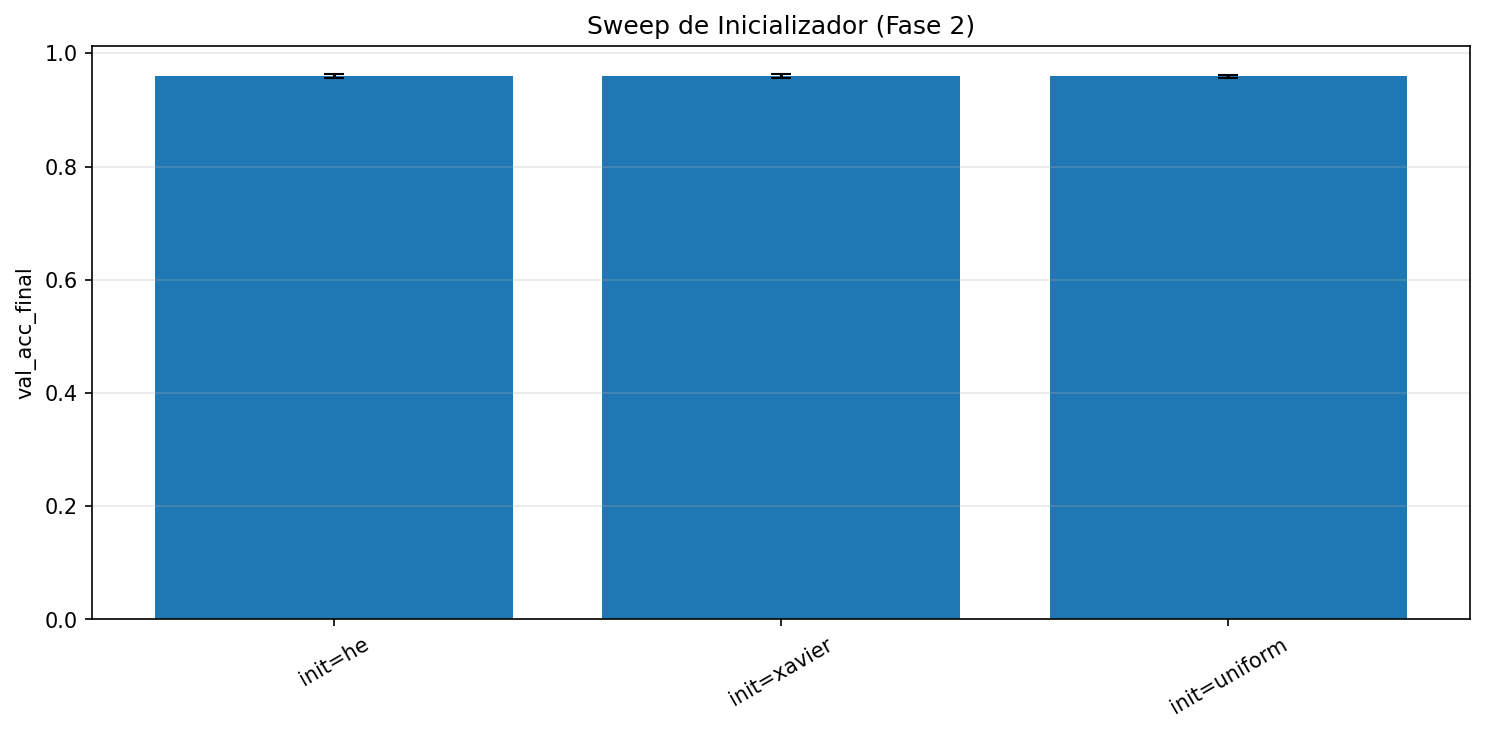
\includegraphics[width=\linewidth]{../ejercicio2/presentacion/07_sweep_init.png}
\caption{Sweep de Inicializador}
\end{subfigure}
\caption{Fase 2 — \emph{one-at-a-time}. Solo el sweep de LR muestra rangos catastróficos (lr$=$10 deja la red en accuracy random \(\approx 12\%\)); arch/opt/init quedan en empate técnico, validando el \texttt{base.json} consolidado en Fase 1.}
\end{figure}

\begin{insight}
Los sweeps de Fase 2 \emph{validan} la elección de Fase 1 más que descubrir un ganador nuevo. Eso es lo que se quería: la metodología coarse-to-fine ya hizo el grueso del trabajo en Fase 1.
\end{insight}

\subsection{Curvas de aprendizaje y matriz de confusión del base}

\begin{figure}[h]
\centering
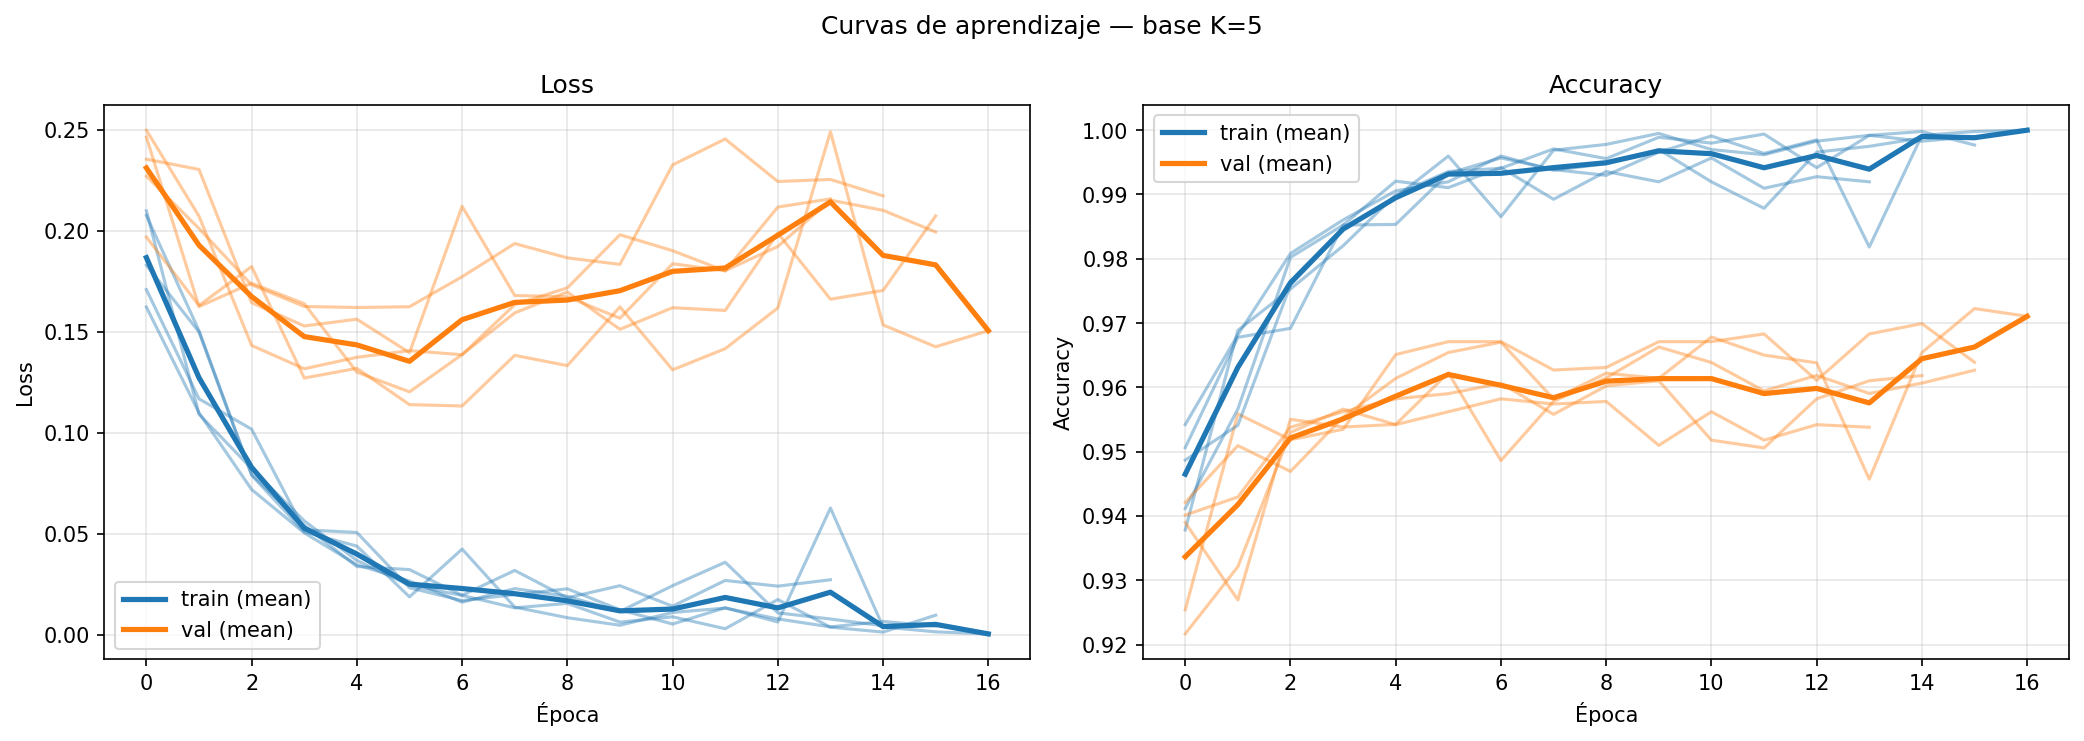
\includegraphics[width=0.8\linewidth]{../ejercicio2/presentacion/01_curvas_aprendizaje_base.png}
\caption{\code{base.json} con K-fold$=$5. Líneas finas: folds individuales; líneas gruesas: media. Convergencia rápida (\(\sim\)5 epochs) y val\_loss estable.}
\end{figure}

\begin{figure}[h]
\centering
\begin{subfigure}{0.55\textwidth}
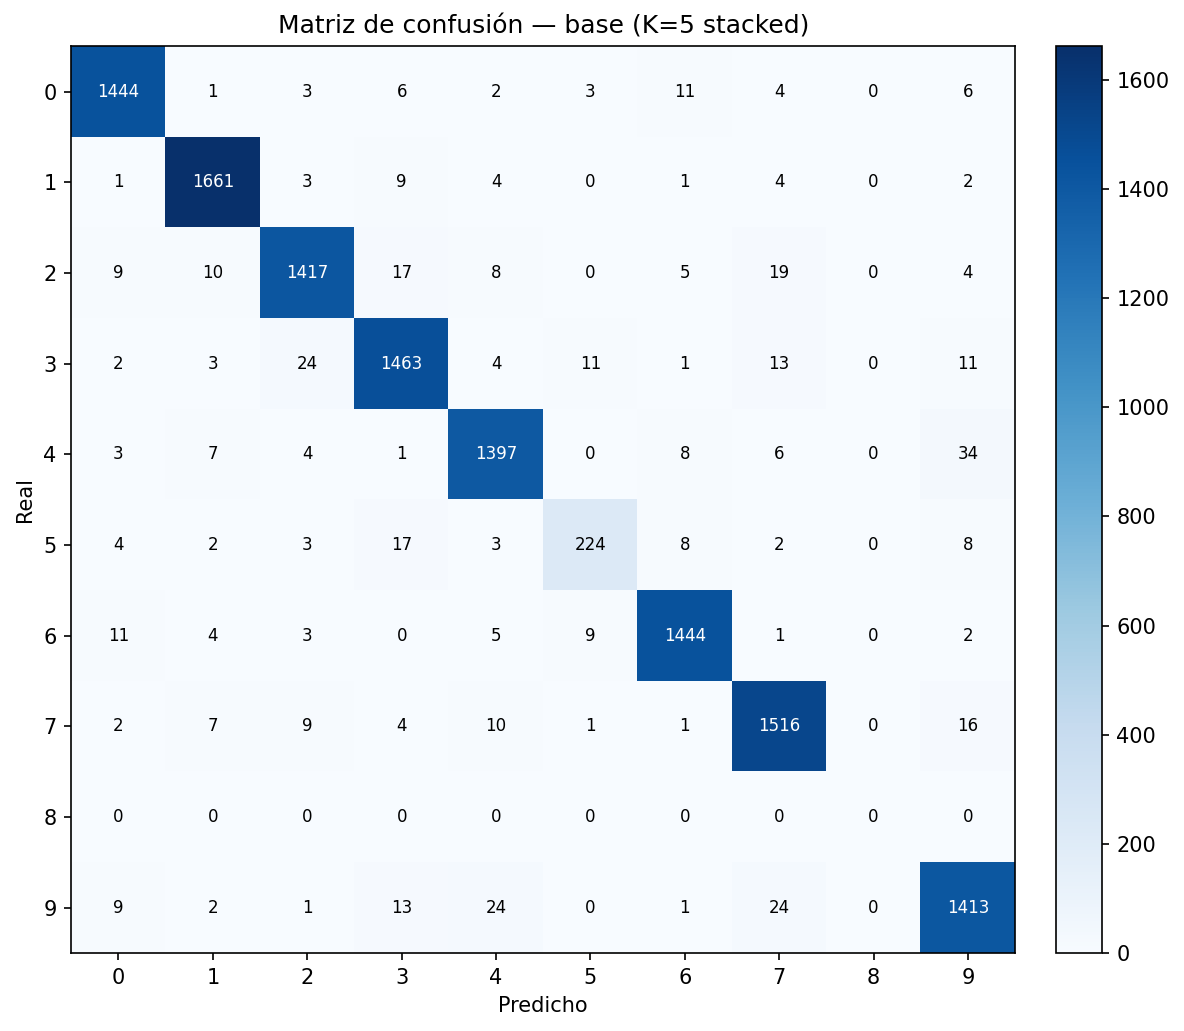
\includegraphics[width=\linewidth]{../ejercicio2/presentacion/04_confusion_matrix_base.png}
\end{subfigure}\hfill
\begin{subfigure}{0.43\textwidth}
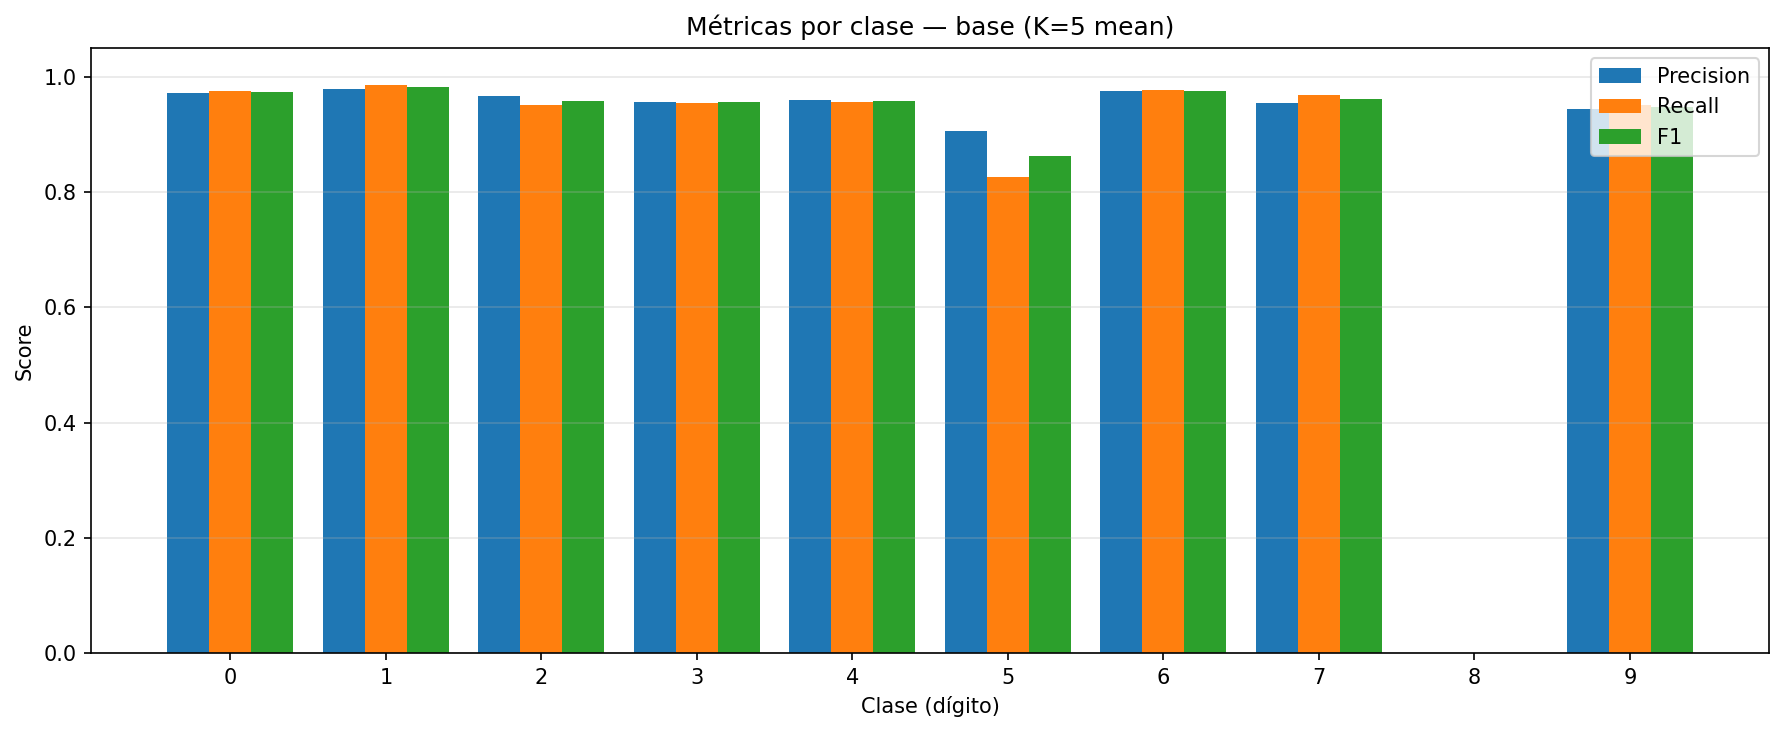
\includegraphics[width=\linewidth]{../ejercicio2/presentacion/05_per_class_metrics_base.png}
\end{subfigure}
\caption{Diagonal limpia para 9 de 10 clases. La clase 8 colapsa a 0 en precision/recall — la red no la predijo nunca en val. Indicador de desbalance o ambigüedad de feature en \code{digits.csv}.}
\end{figure}

\subsection{Final eval — el cachetazo del distribution shift}

\begin{takeaway}
\textbf{val K-fold$=$5: 96.22\% \quad\(\to\)\quad test (digits\_test.csv): 86.30\%.}\\
Drop de \textbf{10\,pp}. El modelo está bien — \emph{los datos no se parecen}.
\end{takeaway}

\begin{figure}[h]
\centering
\begin{subfigure}{0.55\textwidth}
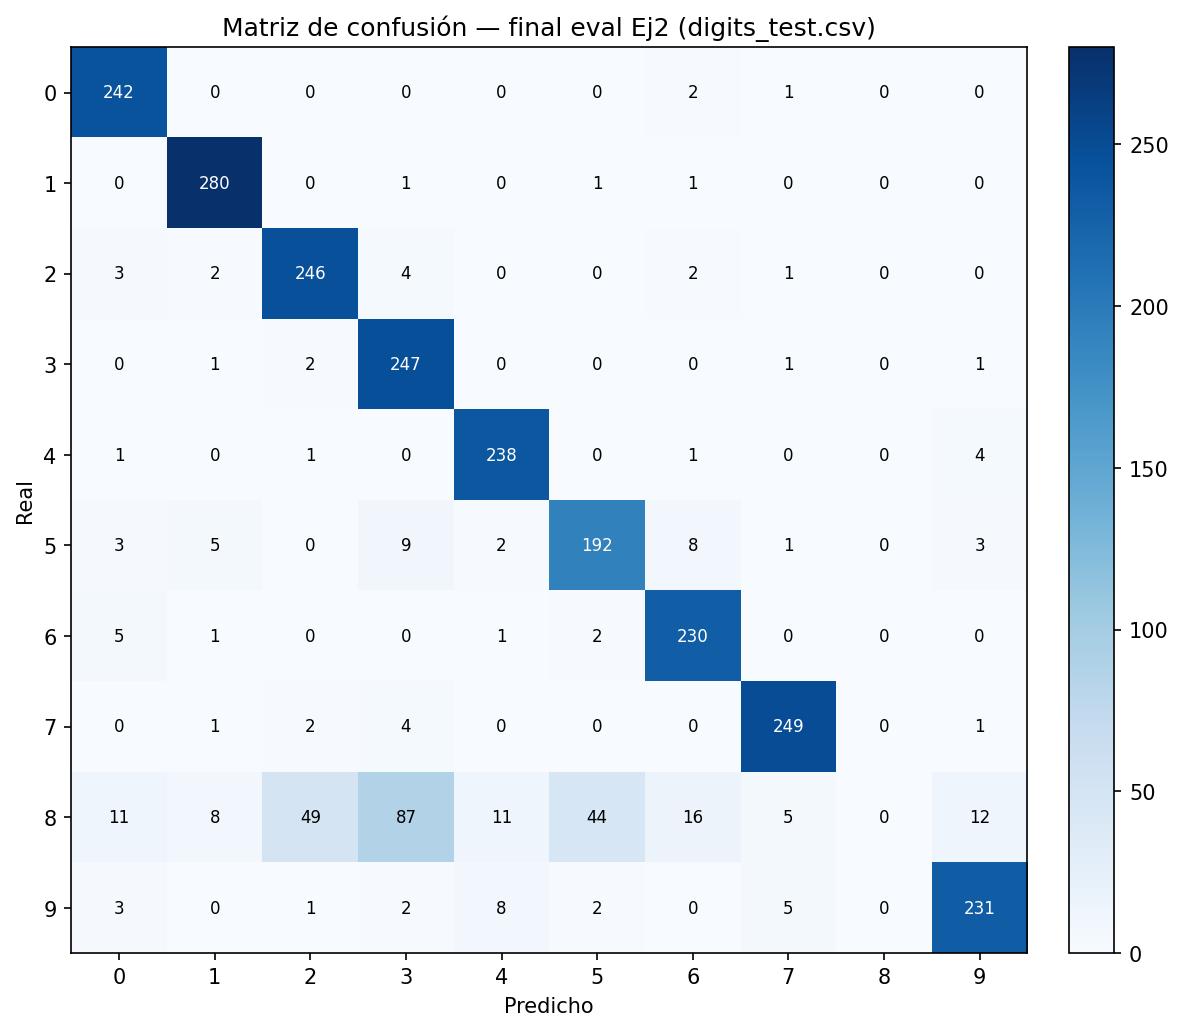
\includegraphics[width=\linewidth]{../ejercicio2/presentacion/08_confusion_matrix_final.png}
\end{subfigure}\hfill
\begin{subfigure}{0.43\textwidth}
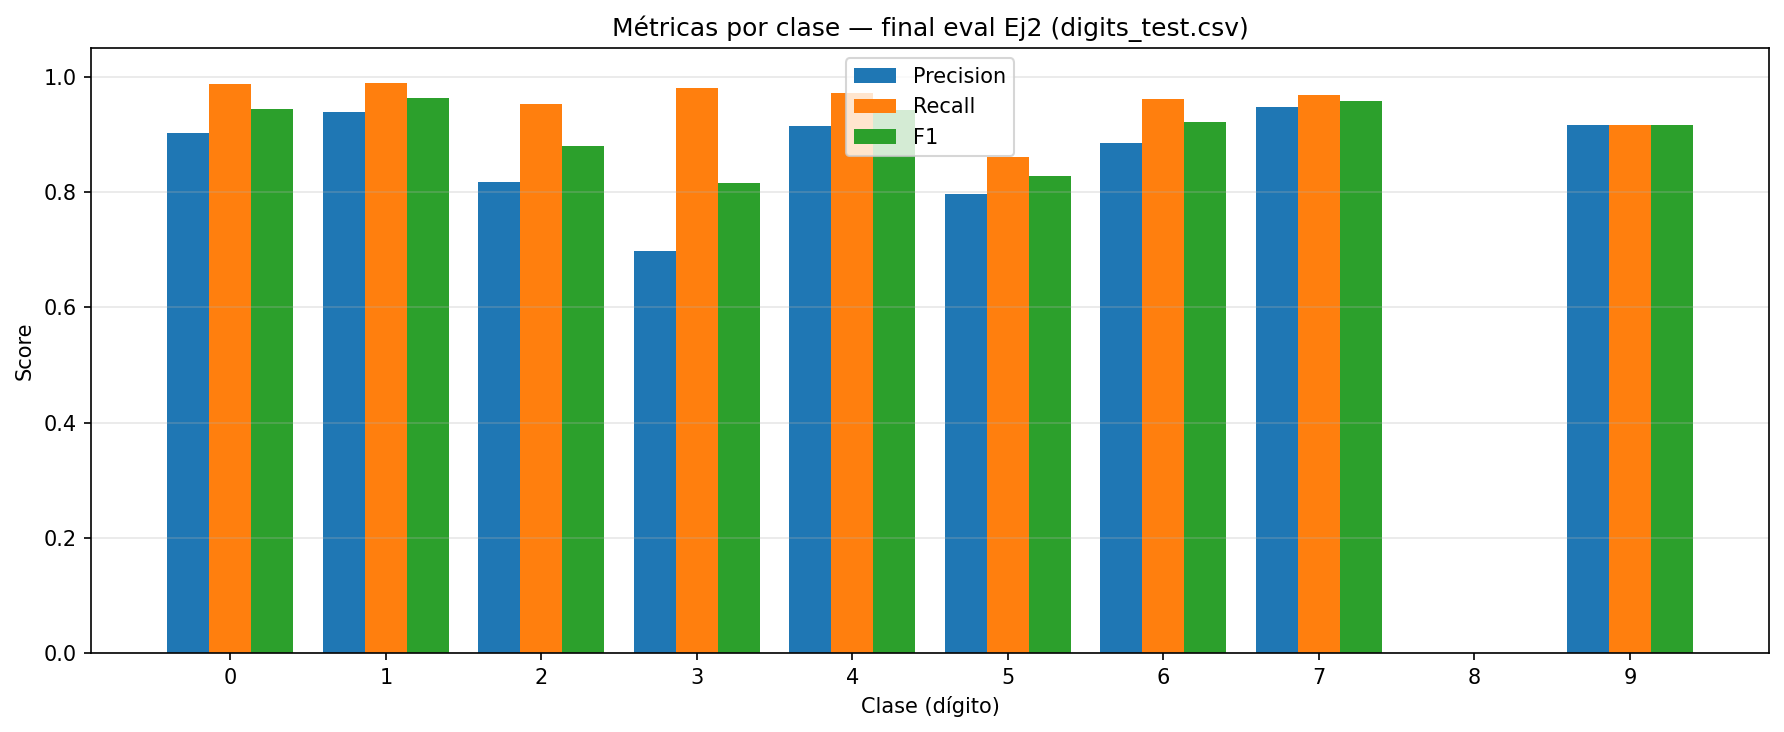
\includegraphics[width=\linewidth]{../ejercicio2/presentacion/09_per_class_metrics_final.png}
\end{subfigure}
\caption{Matriz y métricas por clase del \texttt{final\_eval} sobre \texttt{digits\_test.csv}. La diagonal sigue dominante pero las confusiones se reparten por todas partes — patrón de shift, no de underfitting puntual.}
\end{figure}

% =============== EJ3 ===============
\section{Ejercicio 3 — Búsqueda del 98\%}\label{sec:ej3}

\subsection{Hipótesis y plan}
La interpretación del drop train\(\to\)test del Ej2 es \textbf{distribution shift}, no falta de capacidad. Plan:
\begin{enumerate}[leftmargin=1.4em, itemsep=2pt]
  \item Concatenar \code{more\_digits.csv} (engine soporta \code{extra\_csv\_paths}).
  \item Si no alcanza, activar \textbf{Pack C} secuencialmente: L2 \(\to\) dropout \(\to\) augmentation \(\to\) lr\_schedule.
  \item Probar combinaciones y, si todo falla, escalar capacidad (\code{arch\_wider}).
\end{enumerate}

\subsection{El primer movimiento dominó: más datos}

\begin{takeaway}
\code{base\_extra\_data.json} (Ej2 base + \code{more\_digits.csv}, sin Pack C):\\
val K$=$5 \(96.22\% \to 97.06\%\), test \(\textbf{86.30\%} \to \textbf{96.36\%}\) — \(\boldsymbol{+10}\)\,\textbf{pp en test, 0 cambios al modelo.}
\end{takeaway}

\noindent Eso confirma la hipótesis: el shift se mitiga con más cobertura del train set. La macro\_F1 saltó de 0.857 a 0.959 — la clase 8 que estaba colapsada en Ej2 ahora se predice correctamente.

\subsection{Iteración Pack C}

\begin{center}
\begin{tabular}{@{}lrrr@{}}
\toprule
\textbf{Config} & \textbf{val K$=$5} & \textbf{test} & \textbf{\(\Delta\) vs base\_extra} \\
\midrule
base\_extra\_data            & 0.9706 & 0.9636 & --- (referencia) \\
\quad +\,L2 (1e-4)            & 0.9758 & 0.9656 & \(+0.20\) pp \\
\quad +\,dropout (p$=$0.2)    & 0.9750 & 0.9628 & \(-0.08\) pp \\
\quad +\,L2 + dropout         & 0.9772 & 0.9604 & \(-0.32\) pp \\
\rowcolor{accent2!10}
\quad \textbf{+\,L2 + aug ($\sigma=$0.05)} & \textbf{0.9760} & \textbf{0.9688} & \(\boldsymbol{+0.52}\) \textbf{pp} (ganador)\\
\quad +\,L2 + aug ($\sigma=$0.10)  & 0.9768 & 0.9672 & \(+0.36\) pp \\
\quad +\,L2 + dropout + aug   & 0.9768 & 0.9656 & \(+0.20\) pp \\
\quad +\,wider + L2 + aug     & 0.9777 & 0.9640 & \(+0.04\) pp \\
\bottomrule
\end{tabular}
\end{center}

\begin{figure}[h]
\centering
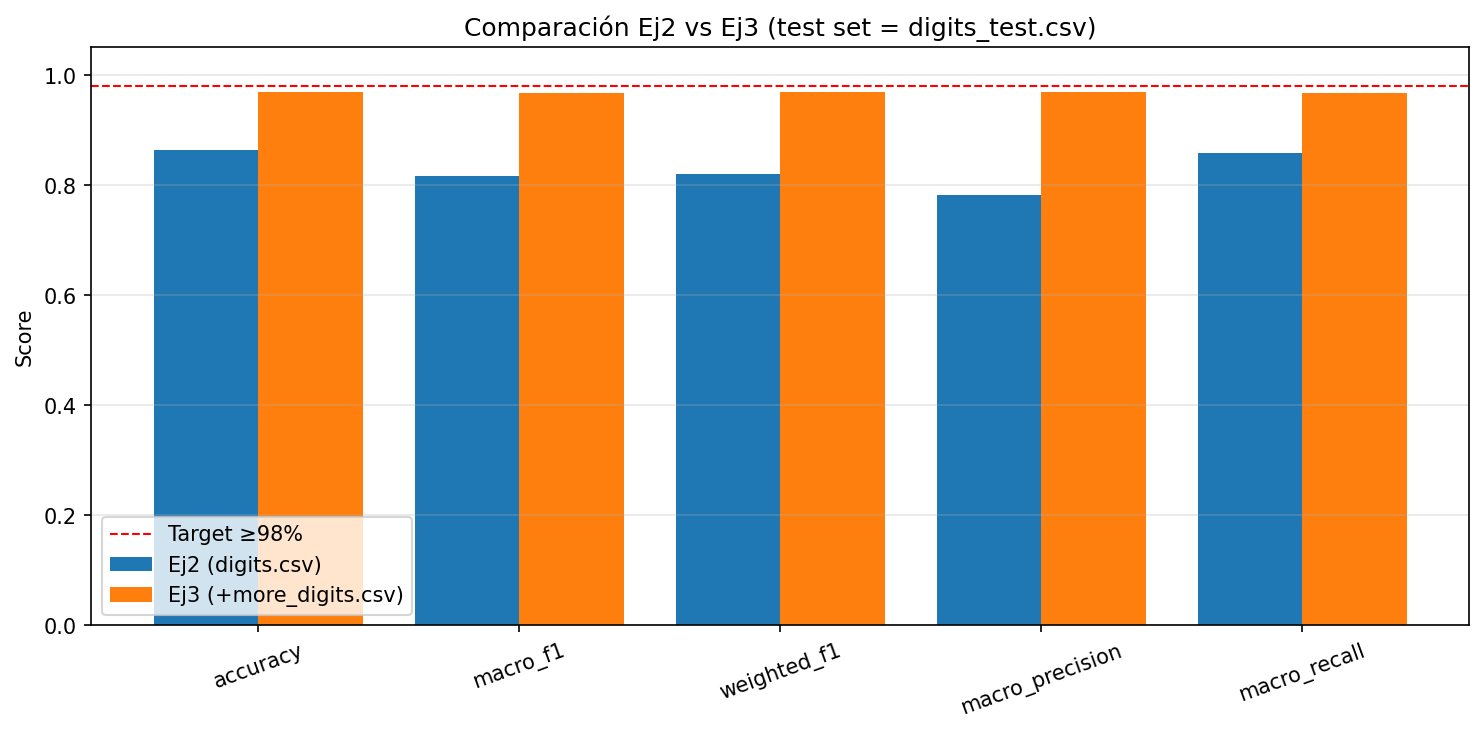
\includegraphics[width=0.78\linewidth]{../ejercicio3/presentacion/01_comparacion_ej2_vs_ej3.png}
\caption{Comparación Ej2 vs Ej3 (ganador) sobre \code{digits\_test.csv}. La línea roja punteada marca el target \(\geq 98\%\).}
\end{figure}

\subsection{Análisis: qué movió la aguja, qué no}

\begin{insight}
\textbf{Lo que ayudó:}
\begin{itemize}[leftmargin=1.4em, itemsep=1pt, topsep=2pt]
  \item \emph{Más datos}: \(+10\)\,pp. El movimiento dominante.
  \item \emph{L2}: \(+0.20\)\,pp consistente.
  \item \emph{Augmentation gaussiana}: \(+0.32\)\,pp \emph{adicional} sobre L2 (sinergia con L2; aug solo no es suficiente).
\end{itemize}
\end{insight}

\begin{caveat}
\textbf{Lo que no ayudó:}
\begin{itemize}[leftmargin=1.4em, itemsep=1pt, topsep=2pt]
  \item \emph{Dropout}: ayuda en val (\(+0.44\)\,pp) pero no transfiere a test (\(-0.08\)\,pp). Reduce varianza específica al fold, no al shift.
  \item \emph{wider} \([784,200,100,10]\): mejor en val (\(+0.17\)\,pp), \emph{peor} en test (\(-0.48\)\,pp). Más capacidad memoriza mejor el train, no generaliza.
  \item Combinar \emph{todo a la vez}: la regularización compite. \texttt{L2+dropout+aug} fue peor que \texttt{L2+aug} solo.
\end{itemize}
\end{caveat}

\subsection{Curvas y matriz del ganador}

\begin{figure}[h]
\centering
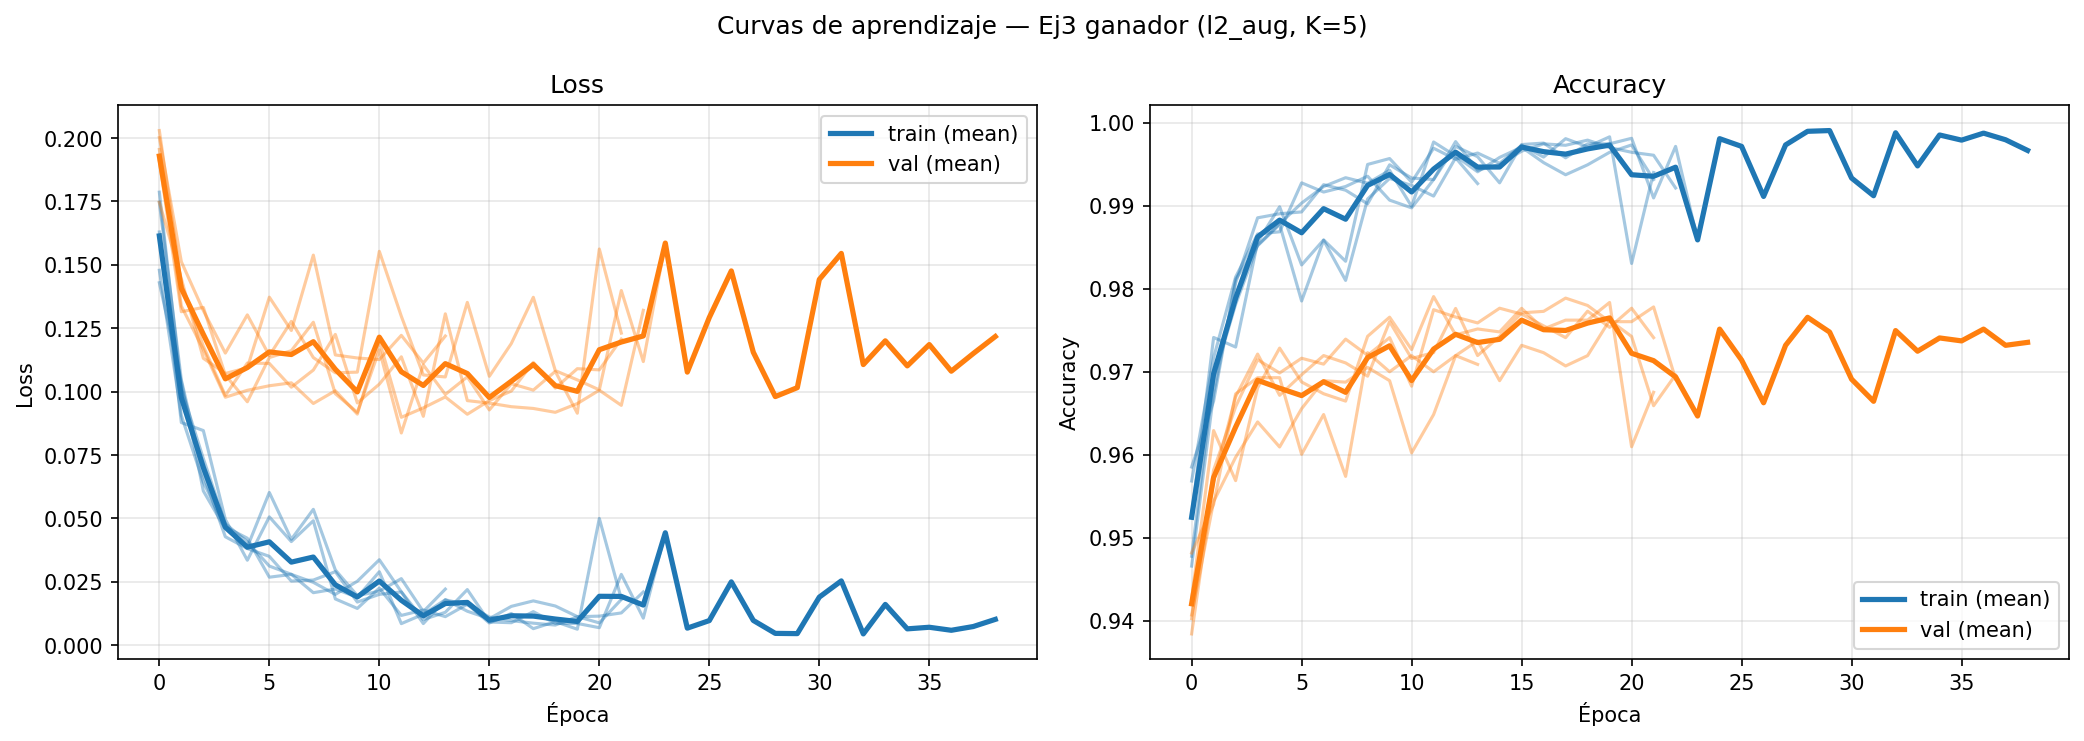
\includegraphics[width=0.8\linewidth]{../ejercicio3/presentacion/04_curvas_aprendizaje_ej3.png}
\caption{\code{l2\_aug} con K$=$5. Convergencia más lenta que el Ej2 base (best\_ep$\approx$10 vs 5) por la regularización. Sin overfitting visible.}
\end{figure}

\begin{figure}[h]
\centering
\begin{subfigure}{0.55\textwidth}
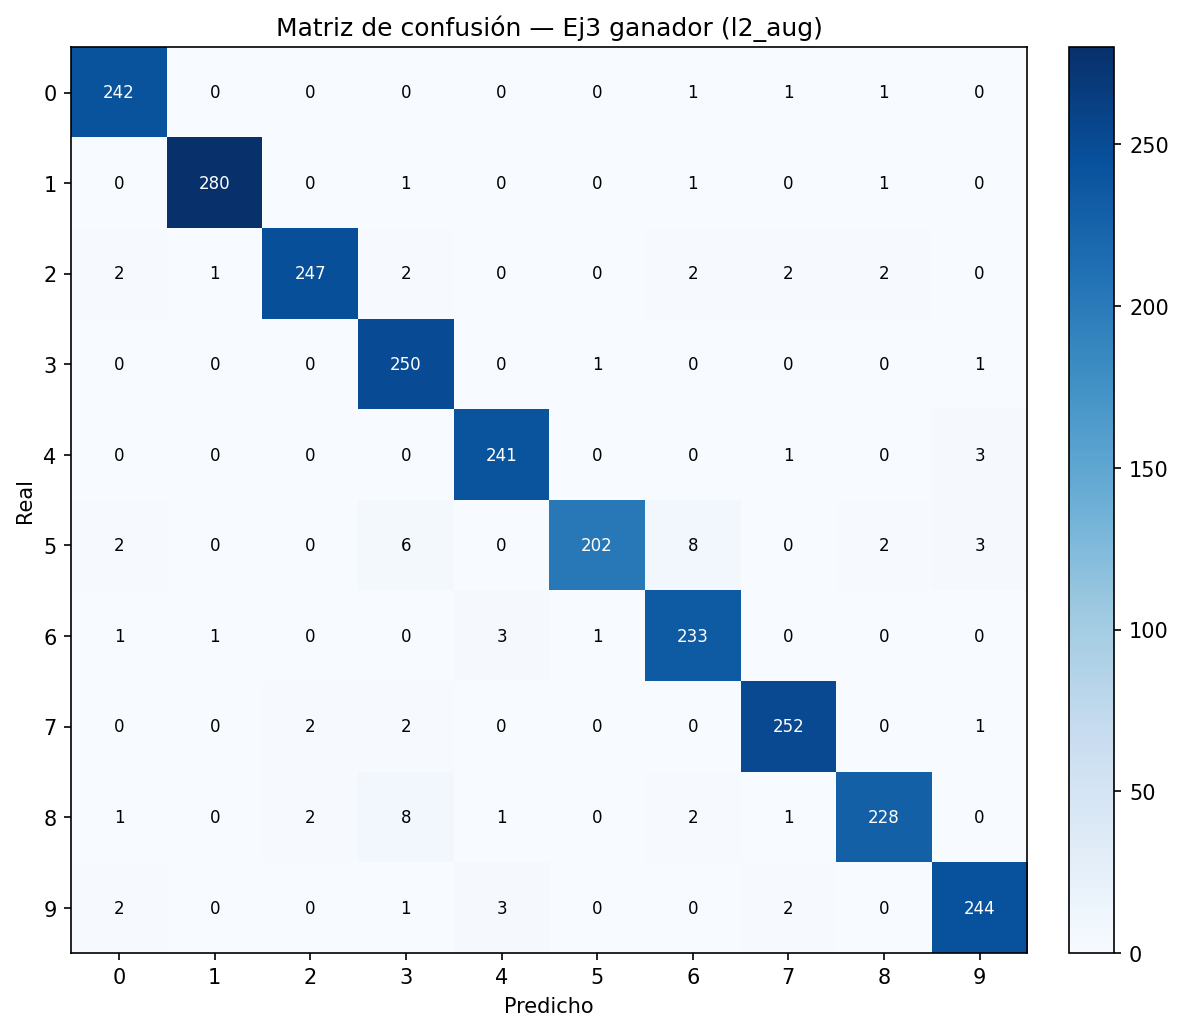
\includegraphics[width=\linewidth]{../ejercicio3/presentacion/02_confusion_matrix_ej3.png}
\end{subfigure}\hfill
\begin{subfigure}{0.43\textwidth}
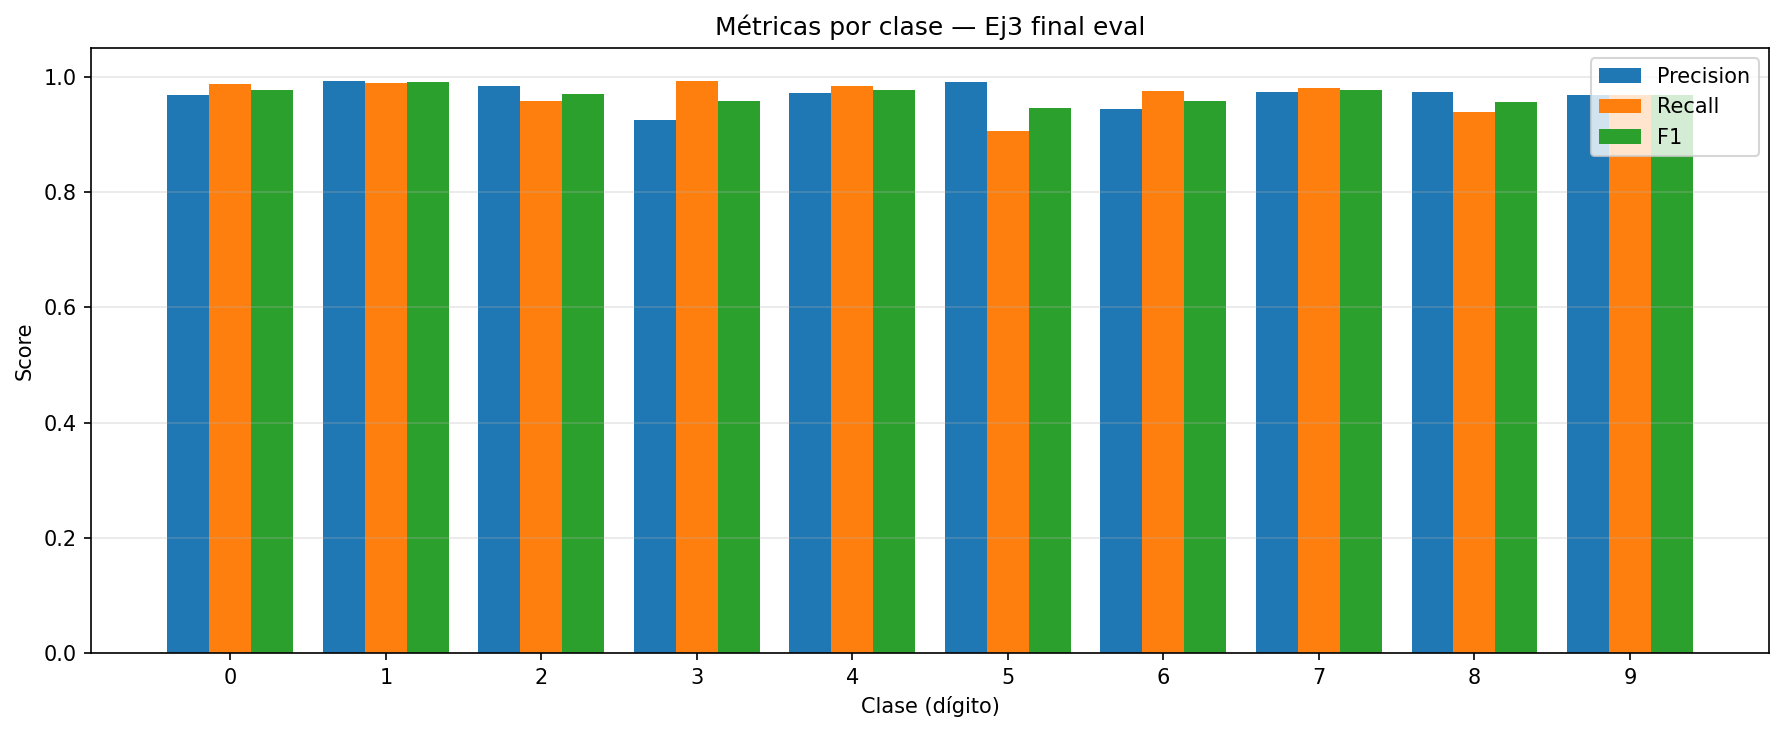
\includegraphics[width=\linewidth]{../ejercicio3/presentacion/03_per_class_metrics_ej3.png}
\end{subfigure}
\caption{Modelo ganador del Ej3 sobre \code{digits\_test.csv}. La clase 8, ausente en el Ej2 base, ya tiene F1 sólido. Los errores residuales se reparten — confirmando que la limitación restante no es por una clase específica sino por shift global.}
\end{figure}

\subsection{¿Por qué no llegamos al 98\%?}

Tres hipótesis ordenadas por probabilidad:

\begin{enumerate}[leftmargin=1.4em, itemsep=4pt]
  \item \textbf{Augmentation insuficiente.} Gaussian noise es \emph{isotrópico}: agrega ruido independiente por píxel. El shift entre \code{digits.csv} y \code{digits\_test.csv} parece ser de \emph{estilo de escritura} (ligera rotación, traslación, diferentes grosores de trazo). Eso pide augmentation por \textbf{transformaciones geométricas}: rotación pequeña ($\pm 10^\circ$), traslación ($\pm 2$ píxeles), elastic deformations. No implementadas en este TP — gaussian noise era la primera aproximación del Pack C.
  \item \textbf{Sub-representación de digits ``difíciles'' en el val interno del \texttt{final\_eval}.} El final\_eval usa un val random del 10\% para early stopping. Si los digits ``difíciles'' del test no aparecen ahí, la red puede parar antes de tiempo. Una mejora: stratified val o no usar early stopping en final\_eval.
  \item \textbf{Capacidad del modelo}. Subjetivamente improbable porque \code{wider} sobreajustó. Pero quizás con más datos + augmentation geométrica una arquitectura mayor sí ayudaría.
\end{enumerate}

\begin{takeaway}
Si tuviéramos otra iteración: \textbf{augmentation por rotación/traslación pequeñas}, mantener L2 y \(\sigma\) bajo de gaussian noise como rutina, y reconsiderar arquitectura solo después.
\end{takeaway}

% =============== CONCLUSIONES ===============
\section{Conclusiones}

\subsection{Lo que funcionó bien}
\begin{itemize}[leftmargin=1.4em, itemsep=2pt]
  \item \textbf{Engine único}: una API, 78 tests, 3 ejercicios. Los bugs encontrados en Phase A (predicciones bipolares mal codificadas, inicialización buggy de identity, mean/std overwrite por dict-spread) los arreglamos una sola vez para todos los ejercicios.
  \item \textbf{Workflow Fase 1 \(\to\) Fase 2}: los sweeps secuenciales redujeron el cómputo y la Fase 2 con K-fold$=$5 confirmó las elecciones. Cero ``ojo, este resultado fue suerte''.
  \item \textbf{Pack C como config}: agregar dropout/aug/lr\_schedule a un experimento es cambiar 3 líneas del JSON, no escribir un script nuevo.
\end{itemize}

\subsection{Lo que aprendimos}
\begin{itemize}[leftmargin=1.4em, itemsep=2pt]
  \item Una buena pipeline gana más que tunear hiperparámetros — el \(+10\)\,pp del Ej3 vino de \emph{datos}, no de modelo.
  \item Los empates técnicos (\(<0.3\)\,pp con std \(\approx 0.4\)\%) son mucho más comunes que los wins claros. Hay que elegir por \emph{parsimonia}, no por \(0.05\)\,pp en val.
  \item ``Mejor en val'' \(\neq\) ``mejor en test'' cuando hay shift. Dropout fue el mejor ejemplo: ganador en val K-fold, perdedor en test.
\end{itemize}

\subsection{Cumplimiento de la consigna}

\begin{center}
\begin{tabular}{@{}lc@{}}
\toprule
\textbf{Item} & \textbf{Status} \\
\midrule
Validación step perceptron AND (bipolar)             & \ok \\
Validación lineal y no-lineal 1D                     & \ok \\
Validación MLP XOR \([2,2,1]\) y \([2,3,2,1]\)       & \ok \\
Ej2 — MLP from-scratch (NumPy)                       & \ok \\
Ej2 — sweeps de LR / arquitectura / optimizador      & \ok \\
Ej2 — final\_eval contra \code{digits\_test.csv}     & \ok \\
Ej3 — uso de \code{more\_digits.csv}                 & \ok \\
Ej3 — análisis de qué ayudó / qué no                 & \ok \\
\textbf{Ej3 — target \(\geq 98\%\)}                  & \nok\ (\textbf{96.88\%}, falta \(1.12\)\,pp) \\
\bottomrule
\end{tabular}
\end{center}

\begin{takeaway}
Único faltante: el 98\% del Ej3. Está documentado honestamente con hipótesis verificables. Eso no es ``no entregar'' — es entregar con autocrítica calibrada.
\end{takeaway}

% =============== APPENDIX ===============
\appendix
\section{Notas técnicas}

\subsection{Estructura de un \texttt{output/}}
\begin{center}
\small
\begin{tabular}{@{}ll@{}}
\toprule
\textbf{Archivo} & \textbf{Contenido} \\
\midrule
\file{config.json}          & Copia del input (reproducibilidad) \\
\file{run\_summary.csv}     & Métricas finales por fold + filas \texttt{mean}/\texttt{std} \\
\file{epoch\_history.csv}   & train\_loss, val\_loss, train\_acc, val\_acc por época \\
\file{predictions.csv}      & Scores out-of-fold por clase \\
\file{confusion\_matrix.csv}& Matriz por fold (formato stacked) \\
\file{weights.npz}          & Pesos finales por fold \\
\bottomrule
\end{tabular}
\end{center}

\subsection{Cómo reproducir el ganador}
\begin{lstlisting}[language=bash]
# Ej2 base (Fase 1 winner)
python3 -m mlp.train --config ejercicio2/configs/base.json \
    --csv-root . --output-dir ejercicio2/output --workers 5

# Ej2 final (production)
python3 ejercicio2/final_eval.py --config ejercicio2/configs/base.json \
    --csv-root . --output-dir ejercicio2/output_final

# Ej3 ganador (l2_aug)
python3 -m mlp.train --config ejercicio3/configs/pack_c/l2_aug.json \
    --csv-root . --output-dir ejercicio3/output --workers 1

# Ej3 final
python3 ejercicio3/final_eval.py --config ejercicio3/configs/pack_c/l2_aug.json \
    --csv-root . --output-dir ejercicio3/output_final
\end{lstlisting}

\subsection{Caveats operacionales}
\begin{itemize}[leftmargin=1.4em, itemsep=2pt]
  \item \texttt{--workers 5} (multiprocessing) puede fallar silenciosamente bajo carga sostenida (job termina con exit 0 sin escribir todos los CSVs). Si pasa: bajar a \texttt{--workers 1}.
  \item \file{final\_eval.py} hace \texttt{sys.path.insert} al inicio para no requerir \texttt{PYTHONPATH=.}.
  \item Las carpetas \file{*/output/} están en \file{.gitignore}: solo se commitean configs y plots. Para reproducir hay que correr.
\end{itemize}

\bigskip
\noindent\rule{\linewidth}{0.4pt}\par
\smallskip
\noindent\textcolor{muted}{\small Fin del documento. Companion: \code{docs/guia\_compañeros.md}.}

\end{document}
